% questions.tex —— 2014 年全国Ⅰ卷（文科） · 题目内容片段（无答案）
% 由 tools/generate_projects.py 依来源总账自 2014/2014_数学真题_全国1文_试题.md 生成，勿手改（改源 MD 后重跑）


\gkpart{数学}

\begin{gktip}
\textbf{来源说明}：本题面依据固定源 PDF 两页 A3 题面逐题转录，原卷印刷页码 901–902。固定源只含试题和作答空白，不附答案或解析；答案和解析均由本库独立复算。

\textbf{图形说明}：第 8、9、16、18、19、22 题的题面图形在 LaTeX 工程中以 TikZ/PGFPlots 矢量源重绘。题面中的图片标记仅为转换器定位这些矢量源的标记，仓库不保存 PNG、JPEG 或 SVG 图形文件。
\end{gktip}

\gkpart{一、选择题}

\begin{question}
\gkti{1}已知集合 $M=\{x\mid -1<x<3\}$，$N=\{x\mid -2<x<1\}$，则 $M\cap N=$\mbox{（　　）}

（A）$(-2,1)$　　（B）$(-1,1)$　　（C）$(1,3)$　　（D）$(-2,3)$

\end{question}
\begin{question}
\gkti{2}若 $\tan\alpha>0$，则\mbox{（　　）}

（A）$\sin2\alpha>0$　　（B）$\cos\alpha>0$　　（C）$\sin\alpha>0$　　（D）$\cos2\alpha>0$

\end{question}
\begin{question}
\gkti{3}设 $z=\dfrac1{1+i}+i$，则 $|z|=$\mbox{（　　）}

（A）$\dfrac12$　　（B）$\dfrac{\sqrt2}{2}$　　（C）$\dfrac{\sqrt3}{2}$　　（D）$2$

\end{question}
\begin{question}
\gkti{4}已知双曲线 $\dfrac{x^2}{a^2}-\dfrac{y^2}{3}=1\ (a>0)$ 的离心率为 $2$，则 $a=$\mbox{（　　）}

（A）$2$　　（B）$\dfrac{\sqrt6}{2}$　　（C）$\dfrac{\sqrt5}{2}$　　（D）$1$

\end{question}
\begin{question}
\gkti{5}设函数 $f(x),g(x)$ 的定义域都为 $\mathbb R$，且 $f(x)$ 是奇函数，$g(x)$ 是偶函数，则下列结论正确的是\mbox{（　　）}

（A）$f(x)|g(x)|$ 是奇函数　　（B）$|f(x)|g(x)$ 是奇函数

（C）$f(x)g(x)$ 是偶函数　　（D）$|f(x)g(x)|$ 是奇函数

\end{question}
\begin{question}
\gkti{6}设 $D,E,F$ 分别为 $\triangle ABC$ 的三边 $BC,CA,AB$ 的中点，则 $\overrightarrow{EB}+\overrightarrow{FC}=$\mbox{（　　）}

（A）$\overrightarrow{BC}$　　（B）$\dfrac12\overrightarrow{AD}$　　（C）$\overrightarrow{AD}$　　（D）$\dfrac12\overrightarrow{BC}$

\end{question}
\begin{question}
\gkti{7}在函数① $y=\cos|2x|$，② $y=|\cos x|$，③ $y=\cos\left(2x+\dfrac\pi6\right)$，④ $y=\tan\left(2x-\dfrac\pi4\right)$ 中，最小正周期为 $\pi$ 的所有函数为\mbox{（　　）}

（A）②④　　（B）①③④　　（C）①②③　　（D）①③

\Needspace{0.4\textheight}
\end{question}
\begin{question}
\gkti{8}如图，网格纸的各小格都是正方形，粗实线画出的是一个几何体的三视图，则这个几何体是\mbox{（　　）}
\nopagebreak[4]
\begin{center}% 2014 全国卷Ⅰ文科第 8 题：方格纸上的三视图。
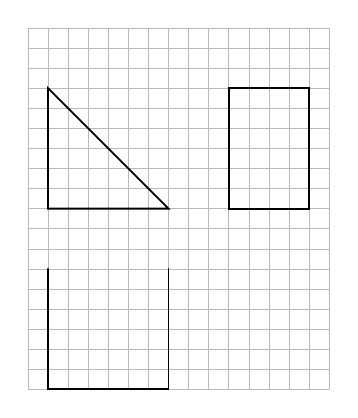
\begin{tikzpicture}[x=2.55mm,y=2.55mm,line cap=round]
  % 细灰色方格；粗实线是题面给出的三个投影。
  \draw[step=1,gray!55,line width=.18pt] (0,0) grid (15,18);
  \draw[line width=.65pt] (1,15)--(1,9)--(7,9)--cycle;
  \draw[line width=.65pt] (10,15)--(14,15)--(14,9)--(10,9)--cycle;
  \draw[line width=.65pt] (1,6)--(1,0)--(7,0)--(7,6);
\end{tikzpicture}
\end{center}
\nopagebreak[4]
（A）三棱锥　　（B）三棱柱　　（C）四棱锥　　（D）四棱柱

\Needspace{0.4\textheight}
\end{question}
\begin{question}
\gkti{9}执行如图的程序框图，若输入的 $a,b,k$ 分别为 $1,2,3$，则输出的 $M=$\mbox{（　　）}
\nopagebreak[4]
\begin{center}% 2014 全国卷Ⅰ文科第 9 题：迭代计算程序框图。
\begin{tikzpicture}[font=\footnotesize,>=Stealth,node distance=4mm,line width=.4pt,
  box/.style={draw,minimum height=1.65em,minimum width=6.4em,inner xsep=5pt},
  term/.style={draw,rounded corners=6pt,minimum height=1.65em,inner xsep=8pt},
  io/.style={draw,trapezium,trapezium left angle=70,trapezium right angle=110,
             minimum height=1.65em,inner xsep=4pt},
  dec/.style={draw,diamond,aspect=2.25,inner sep=1.6pt}]
  \node[term] (start) {开始};
  \node[io,below=of start] (input) {输入 $a,b,k$};
  \node[box,below=of input] (init) {$n=1$};
  \node[dec,below=7mm of init] (cond) {$n\leqslant k$};
  \node[box,below=8mm of cond] (calc) {$M=a+\dfrac1b$};
  \node[box,below=of calc] (seta) {$a=b$};
  \node[box,below=of seta] (setb) {$b=M$};
  \node[box,below=of setb] (inc) {$n=n+1$};
  \node[io,left=23mm of calc] (output) {输出 $M$};
  \node[term,below=of output] (end) {结束};
  \draw[->] (start)--(input)--(init)--(cond);
  \draw[->] (cond)--node[right] {是}(calc)--(seta)--(setb)--(inc);
  \draw[->] (inc.east)-| ([xshift=19mm]cond.east) |- (cond.north);
  \draw[->] (cond.west)-|node[pos=.17,above] {否}(output.north);
  \draw[->] (output)--(end);
\end{tikzpicture}
\end{center}
\nopagebreak[4]
（A）$\dfrac{20}{3}$　　（B）$\dfrac72$　　（C）$\dfrac{16}{5}$　　（D）$\dfrac{15}{8}$

\end{question}
\begin{question}
\gkti{10}已知抛物线 $C:y^2=x$ 的焦点为 $F$，$A(x_0,y_0)$ 是 $C$ 上一点，$|AF|=\dfrac54x_0$，则 $x_0=$\mbox{（　　）}

（A）$4$　　（B）$2$　　（C）$1$　　（D）$8$

\end{question}
\begin{question}
\gkti{11}设 $x,y$ 满足约束条件

\nopagebreak[4]
\[
\begin{cases}
x+y\geqslant a,\\
x-y\leqslant-1,
\end{cases}
\]

且 $z=x+ay$ 的最小值为 $7$，则 $a=$\mbox{（　　）}

（A）$-5$　　（B）$3$　　（C）$-5$ 或 $3$　　（D）$5$ 或 $-3$

\end{question}
\begin{question}
\gkti{12}已知函数 $f(x)=ax^3-3x^2+1$，若 $f(x)$ 存在唯一的零点 $x_0$，且 $x_0>0$，则 $a$ 的取值范围为\mbox{（　　）}

（A）$(-\infty,-2)$　　（B）$(1,+\infty)$　　（C）$(2,+\infty)$　　（D）$(-\infty,-1)$

\end{question}
\gkpart{二、填空题}

\begin{question}
\gkti{13}将 $2$ 本不同的数学书和 $1$ 本语文书在书架上随机排成一行，则 $2$ 本数学书相邻的概率为\gkblank{}。

\end{question}
\begin{question}
\gkti{14}甲、乙、丙三位同学被问到是否去过 $A,B,C$ 三个城市时，甲说：我去过的城市比乙多，但没去过 $B$ 城市；乙说：我没去过 $C$ 城市；丙说：我们三人去过同一个城市。由此可判断乙去过的城市为\gkblank{}。

\end{question}
\begin{question}
\gkti{15}设函数

\nopagebreak[4]
\[
f(x)=\begin{cases}
e^{x-1},&x<1,\\
x^{\frac13},&x\geqslant1,
\end{cases}
\]

则使得 $f(x)\leqslant2$ 成立的 $x$ 的取值范围是\gkblank{}。

\Needspace{0.4\textheight}
\end{question}
\begin{question}
\gkti{16}如图，为测量山高 $MN$，选择 $A$ 和另一座山的山顶 $C$ 为测量观测点。从 $A$ 点测得 $M$ 点的仰角 $\angle MAN=60^\circ$，$C$ 点的仰角 $\angle CAB=45^\circ$ 以及 $\angle MAC=75^\circ$；从 $C$ 点测得 $\angle MCA=60^\circ$。已知山高 $BC=100\ \mathrm m$，则山高 $MN=$\gkblank{} $\mathrm m$。
\nopagebreak[4]
\begin{center}% 2014 全国卷Ⅰ文科第 16 题：测量山高的观测示意图。
\begin{tikzpicture}[font=\footnotesize,line width=.45pt,line cap=round,line join=round]
  \coordinate (A) at (0,0);
  \coordinate (B) at (4.5,0);
  \coordinate (C) at (4.5,2.25);
  \coordinate (N) at (-1.9,.82);
  \coordinate (M) at (-1.9,5.05);
  \draw (M)--(N);
  \draw (B)--(C);
  \draw (A)--(B);
  \draw (A)--(M) (A)--(C) (C)--(M);
  \draw[dashed] (N)--(B);
  \draw[dashed] (N)--(A);
  \node[above] at (M) {$M$};
  \node[left] at (N) {$N$};
  \node[below] at (A) {$A$};
  \node[below] at (B) {$B$};
  \node[right] at (C) {$C$};
\end{tikzpicture}
\end{center}
\nopagebreak[4]
\end{question}
\gkpart{三、解答题}

\begin{question}
\gkti{17}已知 $\{a_n\}$ 是递增的等差数列，$a_2,a_4$ 是方程 $x^2-5x+6=0$ 的根。

(1) 求 $\{a_n\}$ 的通项公式；

(2) 求数列 $\left\{\dfrac{a_n}{2^n}\right\}$ 的前 $n$ 项和。

\Needspace{0.4\textheight}
\end{question}
\begin{question}
\gkti{18}从某企业生产的某种产品中抽取 $100$ 件，测量这些产品的一项质量指标值，由测量结果得如下频数分布表：

\begin{center}
\begin{tabular}{lrrrrr}
\toprule
质量指标值分组 & $[75,85)$ & $[85,95)$ & $[95,105)$ & $[105,115)$ & $[115,125)$ \\
\midrule
频数 & $6$ & $26$ & $38$ & $22$ & $8$ \\
\bottomrule
\end{tabular}
\end{center}

(1) 作出这些数据的频率分布直方图；
\nopagebreak[4]
\begin{center}% 2014 全国卷Ⅰ文科第 18 题：频率分布直方图的待作答空白框。
% 有意不画任何柱条；原题要求考生据频数表自行作图。
\begin{tikzpicture}[font=\scriptsize,>=Stealth,line cap=round]
  \draw[gray!58,line width=.22pt] (.6,0) grid[xstep=1,ystep=.5] (5.6,10);
  \draw[->,line width=.45pt] (-.62,0)--(6.32,0) node[right] {质量指标值};
  \draw[->,line width=.45pt] (0,-.18)--(0,10.72) node[above left,align=center] {频率\\组距};
  % 原点后的断轴锯齿。
  \draw[line width=.4pt] (.14,.10)--(.22,-.10)--(.30,.10)--(.38,-.10)--(.46,.10);
  \foreach \x/\lab in {.6/75,1.6/85,2.6/95,3.6/105,4.6/115,5.6/125}
    \node[below=2pt] at (\x,0) {\lab};
  \node[below=2pt] at (-.38,0) {0};
  \foreach \k in {1,...,20}
    \pgfmathsetmacro\v{\k/500}
    \node[left=2pt] at (0,\k/2) {\pgfmathprintnumber[fixed,fixed zerofill,precision=3]{\v}};
\end{tikzpicture}
\end{center}
\nopagebreak[4]
(2) 估计这种产品质量指标值的平均数及方差（同一组中的数据用该组区间的中点值作代表）；

(3) 根据以上抽样调查数据，能否认为该企业生产的这种产品符合“质量指标值不低于 $95$ 的产品至少要占全部产品的 $80\%$”的规定？

\par\medskip

*以下续自固定源 PDF 第 2 页（印刷页 902）。*

\Needspace{0.4\textheight}
\end{question}
\begin{question}
\gkti{19}如图，三棱柱 $ABC-A_1B_1C_1$ 中，侧面 $BB_1C_1C$ 为菱形，$B_1C$ 的中点为 $O$，且 $AO\perp$ 平面 $BB_1C_1C$。
\nopagebreak[4]
\begin{center}% 2014 全国卷Ⅰ文科第 19 题：三棱柱及侧面内的中点 O。
\begin{tikzpicture}[font=\footnotesize,line width=.45pt,line cap=round,line join=round]
  \coordinate (B) at (0,0);
  \coordinate (C) at (1.55,.82);
  \coordinate (B1) at (3.20,0);
  \coordinate (C1) at (4.70,.82);
  \coordinate (A) at (1.72,2.72);
  \coordinate (A1) at (4.92,2.72);
  \coordinate (O) at ($(B1)!0.5!(C)$);
  \draw (B)--(A)--(B1)--(A1)--(C1)--(B1);
  \draw (A)--(A1) (B1)--(C1) (B)--(B1);
  \draw[dashed] (B)--(C)--(A) (C)--(C1) (C)--(B1) (A)--(O);
  \node[below left] at (B) {$B$};
  \node[left] at (C) {$C$};
  \node[below] at (B1) {$B_1$};
  \node[right] at (C1) {$C_1$};
  \node[above] at (A) {$A$};
  \node[above] at (A1) {$A_1$};
  \node[below left] at (O) {$O$};
\end{tikzpicture}
\end{center}
\nopagebreak[4]
(1) 证明：$B_1C\perp AB$；

(2) 若 $AC\perp AB_1$，$\angle CBB_1=60^\circ$，$BC=1$，求三棱柱 $ABC-A_1B_1C_1$ 的高。

\end{question}
\begin{question}
\gkti{20}已知点 $P(2,2)$，圆 $C:x^2+y^2-8y=0$，过点 $P$ 的动直线 $l$ 与圆 $C$ 交于 $A,B$ 两点，线段 $AB$ 的中点为 $M$，$O$ 为坐标原点。

(1) 求 $M$ 的轨迹方程；

(2) 当 $|OP|=|OM|$ 时，求 $l$ 的方程及 $\triangle POM$ 的面积。

\end{question}
\begin{question}
\gkti{21}设函数 $f(x)=a\ln x+\dfrac{1-a}{2}x^2-bx\ (a\ne1)$，曲线 $y=f(x)$ 在点 $(1,f(1))$ 处的切线斜率为 $0$。

(1) 求 $b$；

(2) 若存在 $x_0\geqslant1$ 使得 $f(x_0)<\dfrac{a}{a-1}$，求 $a$ 的取值范围。

\Needspace{0.4\textheight}
\end{question}
\begin{question}
\gkti{22}如图，四边形 $ABCD$ 是 $\odot O$ 的内接四边形，$AB$ 的延长线与 $DC$ 的延长线交于点 $E$，且 $CB=CE$。
\nopagebreak[4]
\begin{center}% 2014 全国卷Ⅰ文科第 22 题：圆内接四边形、延长线及辅助线。
% 解析自检：A、B、C、D 均取在圆心 O=(0,0)、半径 R=2.4 的圆上；
% A、B 同高，E 是 AB 与 DC 的交点，M 是 AD 中点且 MB=MC。
\begin{tikzpicture}[font=\footnotesize,line width=.45pt,line cap=round,line join=round]
  \coordinate (O) at (0,0);
  \coordinate (A) at (-1.673798076233,-1.720000000000);
  \coordinate (D) at (.621165708246,2.318221983094);
  \coordinate (M) at ($ (A)!0.5!(D) $);
  \coordinate (B) at (1.673798076233,-1.720000000000);
  \coordinate (C) at (2.334272376364,-.557828354374);
  \coordinate (E) at (3.026514778968,-1.720000000000);
  \draw (O) circle (2.4);
  \draw (A)--(D)--(C)--(B)--cycle;
  \draw (A)--(E);
  \draw (D)--(E);
  \draw (M)--(B) (M)--(C);
  \fill (O) circle (1.15pt);
  \node[below left] at (A) {$A$};
  \node[below] at (B) {$B$};
  \node[right] at (C) {$C$};
  \node[above] at (D) {$D$};
  \node[right] at (E) {$E$};
  \node[left] at (M) {$M$};
  \node[below left] at (O) {$O$};
\end{tikzpicture}
\end{center}
\nopagebreak[4]
(1) 证明：$\angle D=\angle E$；

(2) 设 $AD$ 不是 $\odot O$ 的直径，$AD$ 的中点为 $M$，且 $MB=MC$，证明：$\triangle ADE$ 为等边三角形。

\end{question}
\begin{question}
\gkti{23}已知曲线 $C:\dfrac{x^2}{4}+\dfrac{y^2}{9}=1$，直线 $l:\begin{cases}x=2+t,\\y=2-2t,\end{cases}$（$t$ 为参数）。

(1) 写出曲线 $C$ 的参数方程，直线 $l$ 的普通方程；

(2) 过曲线 $C$ 上任一点 $P$ 作与 $l$ 夹角为 $30^\circ$ 的直线，交 $l$ 于点 $A$，求 $|PA|$ 的最大值与最小值。

\end{question}
\begin{question}
\gkti{24}若 $a>0,b>0$，且 $\dfrac1a+\dfrac1b=\sqrt{ab}$。

(1) 求 $a^3+b^3$ 的最小值；

(2) 是否存在 $a,b$，使得 $2a+3b=6$？并说明理由。

\end{question}